% Intended LaTeX compiler: pdflatex
\documentclass[11pt, a4paper]{article}
\usepackage[a4paper, margin=2.2cm]{geometry}
\usepackage[scaled]{helvet}\renewcommand{\familydefault}{\sfdefault}
\usepackage[T1]{fontenc}\usepackage{microtype}\usepackage{graphicx}\usepackage{float}\usepackage{booktabs}
\usepackage{xcolor}\usepackage{enumitem}\usepackage{amssymb}\usepackage{needspace}
\usepackage[nobottomtitles*]{titlesec}\usepackage{caption}
\usepackage{tikz}\usetikzlibrary{positioning, arrows.meta, calc}
\usepackage{tabularx}\newcolumntype{Y}{>{\raggedright\arraybackslash}X}\usepackage{newunicodechar}\newunicodechar{→}{\ensuremath{\rightarrow}}
\usepackage[hidelinks]{hyperref}
\pdftrailerid{}\hyphenpenalty=10000\exhyphenpenalty=10000\setlength{\parindent}{0pt}\setlength{\parskip}{0.5em}
\setlist{itemsep=0.15em, topsep=0.2em, parsep=0pt}\captionsetup{font=small, labelfont=bf}
\definecolor{ink2}{HTML}{52514E}\definecolor{accent}{HTML}{2A78D6}\definecolor{critical}{HTML}{D03B3B}
\definecolor{warm}{HTML}{EB6834}\definecolor{neutral}{HTML}{F0EFEC}\definecolor{band1}{HTML}{FDEBD3}\definecolor{band2}{HTML}{FADBD8}
\tikzset{stage/.style={rounded corners=4pt, draw=accent, line width=1.1pt, fill=white, align=center, font=\small, text width=2.5cm, inner sep=4pt, minimum height=1.25cm},
pstage/.style={stage, dashed, draw=ink2}, ctx/.style={stage, draw=none, fill=neutral},
flow/.style={-{Latex[length=2.4mm]}, line width=0.9pt, draw=ink2}, dflow/.style={flow, dashed}}
\titleformat{\section}{\Large\bfseries}{\thesection}{0.6em}{}\titlespacing*{\section}{0pt}{1.1em}{0.4em}
\titleformat{\subsection}{\large\bfseries\color{accent}}{\thesubsection}{0.5em}{}
\author{Chimdi Walter Ndubuisi, University of Missouri}
\date{19 October 2026 · REVIEW DRAFT for collaborator review, not for circulation}
\title{Learning What to Change: the science-first poster, explained\\\medskip
\large Speaker explainer for poster\_science\_first\_review.pdf}
\begin{document}

\maketitle
\raggedright

\textbf{How to use this.} Read the plain text aloud when presenting. Every figure is reproduced from recorded, hash-pinned
data, or it says ILLUSTRATIVE on its face. Every number comes from the claim ledger
(\texttt{records/CORA\_SUMMIT\_CLAIM\_LEDGER\_20261017.md}), with its scope. The poster is a review draft for Toni, Chris and
Pierce; nothing here is a print-approved claim.

\section{The question, and why it is hard}
\label{sec-question}
\textbf{The general question.} How can a machine learn the objects, relationships and rules in unfamiliar data, and know what to
reconsider when its explanation is not enough? The hard part is not only solving a problem. Before any rule can be
found, the system must decide what the entities are and how they relate. After a rule is found, it must tell whether
the rule really explains the observations, and when it does not, which part of its explanation to change.

This is a research question, not an achievement. The system described here, CORA, makes parts of it executable and
measurable in one controlled setting. It has not solved the general problem, and it has not been applied to biology.

\textbf{The 20-second version.} I study how a reasoning system can tell what to change when its explanation is not good
enough: the objects it sees, the rule it uses, or simply the evidence it has. CORA solves ARC puzzles by writing small
programs. It once built a new rule on a real puzzle and checked it carefully, but a version that ignored its failure
record did the same, and on 58 more puzzles construction added nothing. The measured bottleneck is proposing a usable
rule at all. Whether a system can learn which part of an explanation to revise is the open question.

\textbf{The 90-second version.} Start at the top of the poster with the question and the leaf. Then follow the loop from left to
right: observations, objects, executable rules, testing, and the decision whether the account is supported. Point to the
two shaded bottlenecks. Then show the ARC grids: what a task is, the rule CORA built, and the 0 of 58. End with the
dashed box: a learned prior inside CORA's own search, proposed and not yet validated. Full scripts:
\texttt{POSTER\_90S\_SCIENCE\_FIRST.md} and \texttt{POSTER\_3MIN\_SCIENCE\_FIRST.md}.

\section{A biological motivation}
\label{sec-biology}
The poster's leaf is an \textbf{illustrative schematic}, not a photograph and not data. It stands for a common situation in
biology. Maize lesion-mimic plants form spots of dead tissue without a pathogen. An image shows where and how the lesions
form: their size, spacing and spread. It does not show which biological process produces them.

\begin{itemize}
\item \textbf{Pattern is not mechanism.} Image geometry and topology constrain the possibilities. Naming a process would need
independent molecular or perturbation evidence.
\item \textbf{The entities are part of the inference.} Should the unit be a lesion, a cluster of lesions, a leaf region, a cell
state or a plant? The answer changes which rule can be stated at all.
\item \textbf{The level of inference matters.} Conclusions drawn at the level of single measurements, of individuals, or of
experimental conditions can disagree. A trustworthy system must say at which level a claim holds.
\item \textbf{Independent checks decide.} An explanation that fits the images is a hypothesis. It becomes evidence only when it
predicts something checked independently.
\end{itemize}

No biological pathway, mechanism or molecular result is claimed here. Any biological test would be designed with the
collaborators who hold the data and the domain knowledge (section \ref{sec-people}).

\section{The reasoning loop and its two bottlenecks}
\label{sec-pipeline}
\begin{figure}[H]
\centering
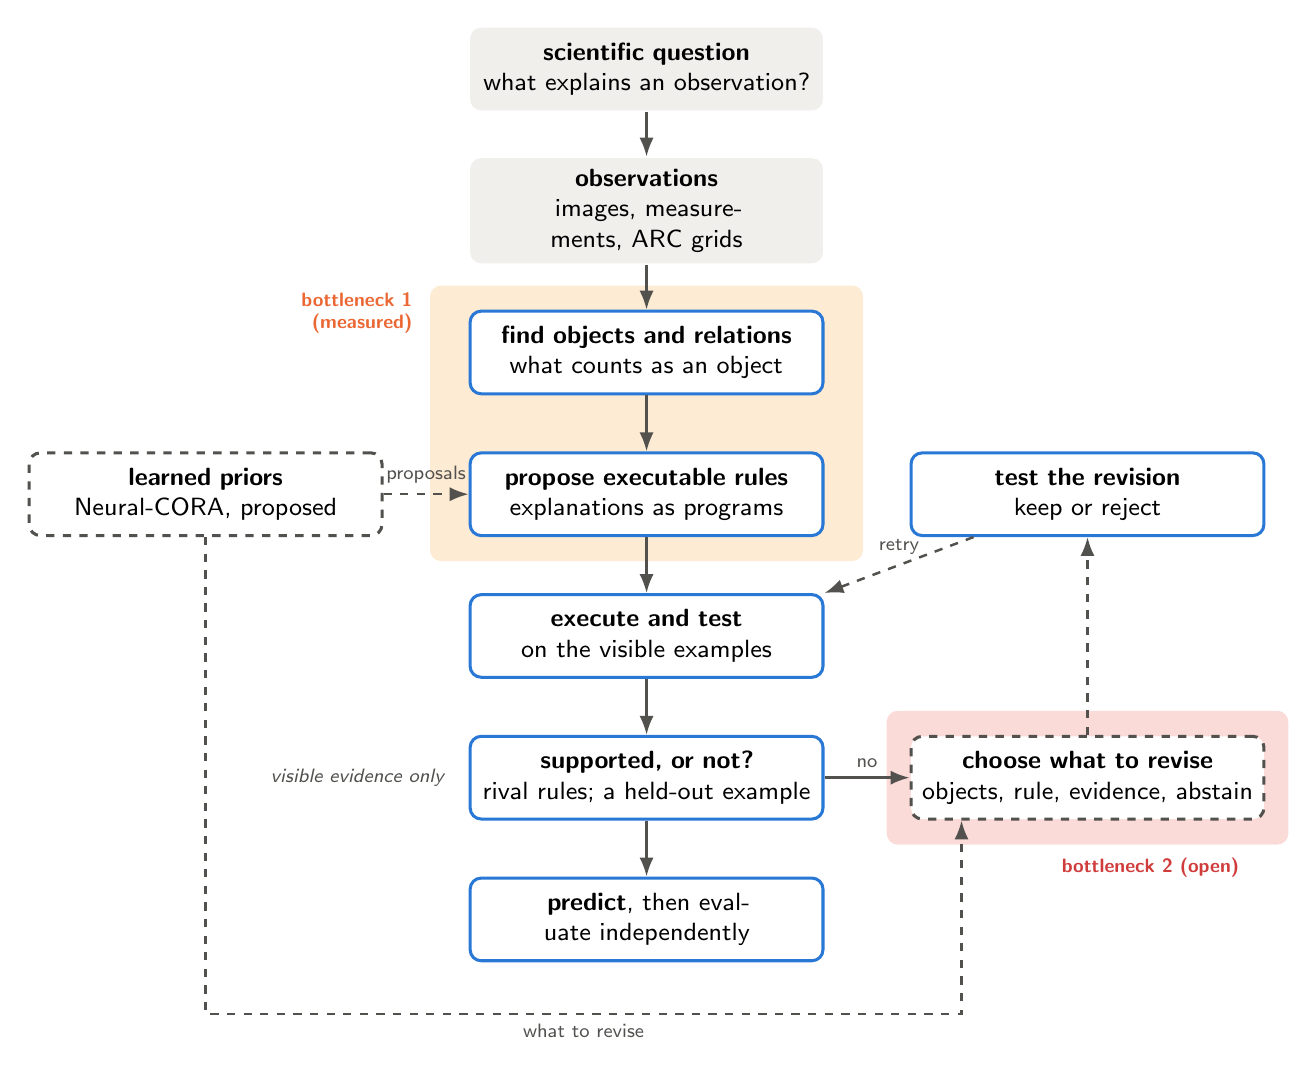
\begin{tikzpicture}
  \tikzset{n/.style={stage, text width=4.2cm, minimum height=1.05cm}, pn/.style={pstage, text width=4.2cm, minimum height=1.05cm},
           cn/.style={ctx, text width=4.2cm, minimum height=1.05cm}}
  \fill[band1, rounded corners=4pt] (-2.75,-6.25) rectangle (2.75,-2.75);
  \fill[band2, rounded corners=4pt] (3.05,-9.85) rectangle (8.15,-8.15);
  \node[cn] (q) at (0,0) {\textbf{scientific question}\\what explains an observation?};
  \node[cn] (o) at (0,-1.8) {\textbf{observations}\\images, measurements, ARC grids};
  \node[n] (f) at (0,-3.6) {\textbf{find objects and relations}\\what counts as an object};
  \node[n] (p) at (0,-5.4) {\textbf{propose executable rules}\\explanations as programs};
  \node[n] (e) at (0,-7.2) {\textbf{execute and test}\\on the visible examples};
  \node[n] (s) at (0,-9.0) {\textbf{supported, or not?}\\rival rules; a held-out example};
  \node[n] (v) at (0,-10.8) {\textbf{predict}, then evaluate independently};
  \foreach \a/\b in {q/o, o/f, f/p, p/e, e/s, s/v} \draw[flow] (\a) -- (\b);
  \node[pn] (r) at (5.6,-9.0) {\textbf{choose what to revise}\\objects, rule, evidence, abstain};
  \node[n] (t) at (5.6,-5.4) {\textbf{test the revision}\\keep or reject};
  \node[pn] (l) at (-5.6,-5.4) {\textbf{learned priors}\\Neural-CORA, proposed};
  \draw[flow] (s) -- node[above, font=\scriptsize, text=ink2] {no} (r);
  \draw[dflow] (r) -- (t);
  \draw[dflow] (t) -- node[above, font=\scriptsize, text=ink2] {retry} (e.north east);
  \draw[dflow] (l) -- node[above, font=\scriptsize, text=ink2] {proposals} (p);
  \draw[dflow] (l.south) -- (-5.6,-12.0) -| node[pos=0.25, below, font=\scriptsize, text=ink2] {what to revise} ($(r.south)+(-1.6,0)$);
  \node[font=\scriptsize\bfseries, text=warm, anchor=east, align=right] at (-2.85,-3.1) {bottleneck 1\\(measured)};
  \node[font=\scriptsize\bfseries, text=critical, anchor=north] at (6.4,-9.9) {bottleneck 2 (open)};
  \node[font=\scriptsize\itshape, text=ink2, anchor=east] at (-2.45,-9.0) {visible evidence only};
\end{tikzpicture}
\caption{\label{fig:pipeline}The poster's reasoning loop. Solid: implemented and tested in CORA. Dashed: proposed or not yet validated. Grey: context, not a CORA component. Shading marks the two bottlenecks.}
\end{figure}

The loop in figure \ref{fig:pipeline} is the poster's main figure. Each arrow means:

\begin{enumerate}
\item \textbf{Scientific question → observations.} A question picks the data: images, molecular measurements, or, in this work, ARC
input and output grids. Grey boxes are context, not parts of CORA.
\item \textbf{Find objects and relations.} Decide what counts as an object and which relations matter. In CORA this is one of seven
segmentation views of a grid. This is the \textbf{representation}.
\item \textbf{Propose executable rules.} Write an explanation as a program that can be run: a \textbf{rule}. CORA proposes programs by
searching its typed language, by native induction from object changes, or by constructing a missing operation.
\item \textbf{Execute and test.} Run each rule on every demonstration. A rule that reproduces every demonstration exactly \textbf{fits}.
\item \textbf{Supported, or not?} A fitting rule may still be unsupported. Rival rules may fit and disagree on the new input, or a
rule may fail when one demonstration is held out and rebuilt from the rest (\textbf{insufficient evidence}). This decision
uses visible evidence only: CORA never sees the hidden test answer.
\item \textbf{Predict, then evaluate independently.} A supported rule predicts the new output. A separate evaluator, which alone
reads the answers, scores it later.
\item \textbf{Choose what to revise.} If the account is incomplete, conflicting or fragile, decide whether to change the objects,
the rule, or the evidence and search, or to abstain. This choice is \textbf{not} validated (dashed).
\item \textbf{Test the revision.} Install the change reversibly, re-test it, and keep it only if it passes the same checks. A
tested revision is not automatically a correct explanation.
\item \textbf{Learned priors (proposed).} A trained model would rank proposals and revisions \textbf{inside} this loop. It never
produces an answer by itself (section \ref{sec-neural}).
\end{enumerate}

\textbf{Bottleneck 1 is measured.} Most failures happen before any test: CORA often cannot propose a usable rule. On 58
separately selected tasks, construction proposed no rule for 55 (section \ref{sec-negative}). \textbf{Bottleneck 2 is open.} Even
when a failure is visible, nothing yet shows that a system can learn which part to revise better than strong blind
alternatives.

An observable diagnostic is not knowledge of the hidden answer. CORA can see that two of its rules disagree, or that one
demonstration alone supports a rule. It cannot see whether its prediction is right.

\section{Why ARC-AGI-2 is the testbed}
\label{sec-arc}
ARC-AGI-2 is a deliberately simplified environment. Each task gives two to five demonstration pairs (an input grid and
its output grid) and one new input. The solver must produce the new output exactly, with two attempts. The answer is
exact, the evidence is small, and every rule can be executed and checked, so representation, rule and evidence can be
studied one at a time.

\begin{figure}[H]
\centering
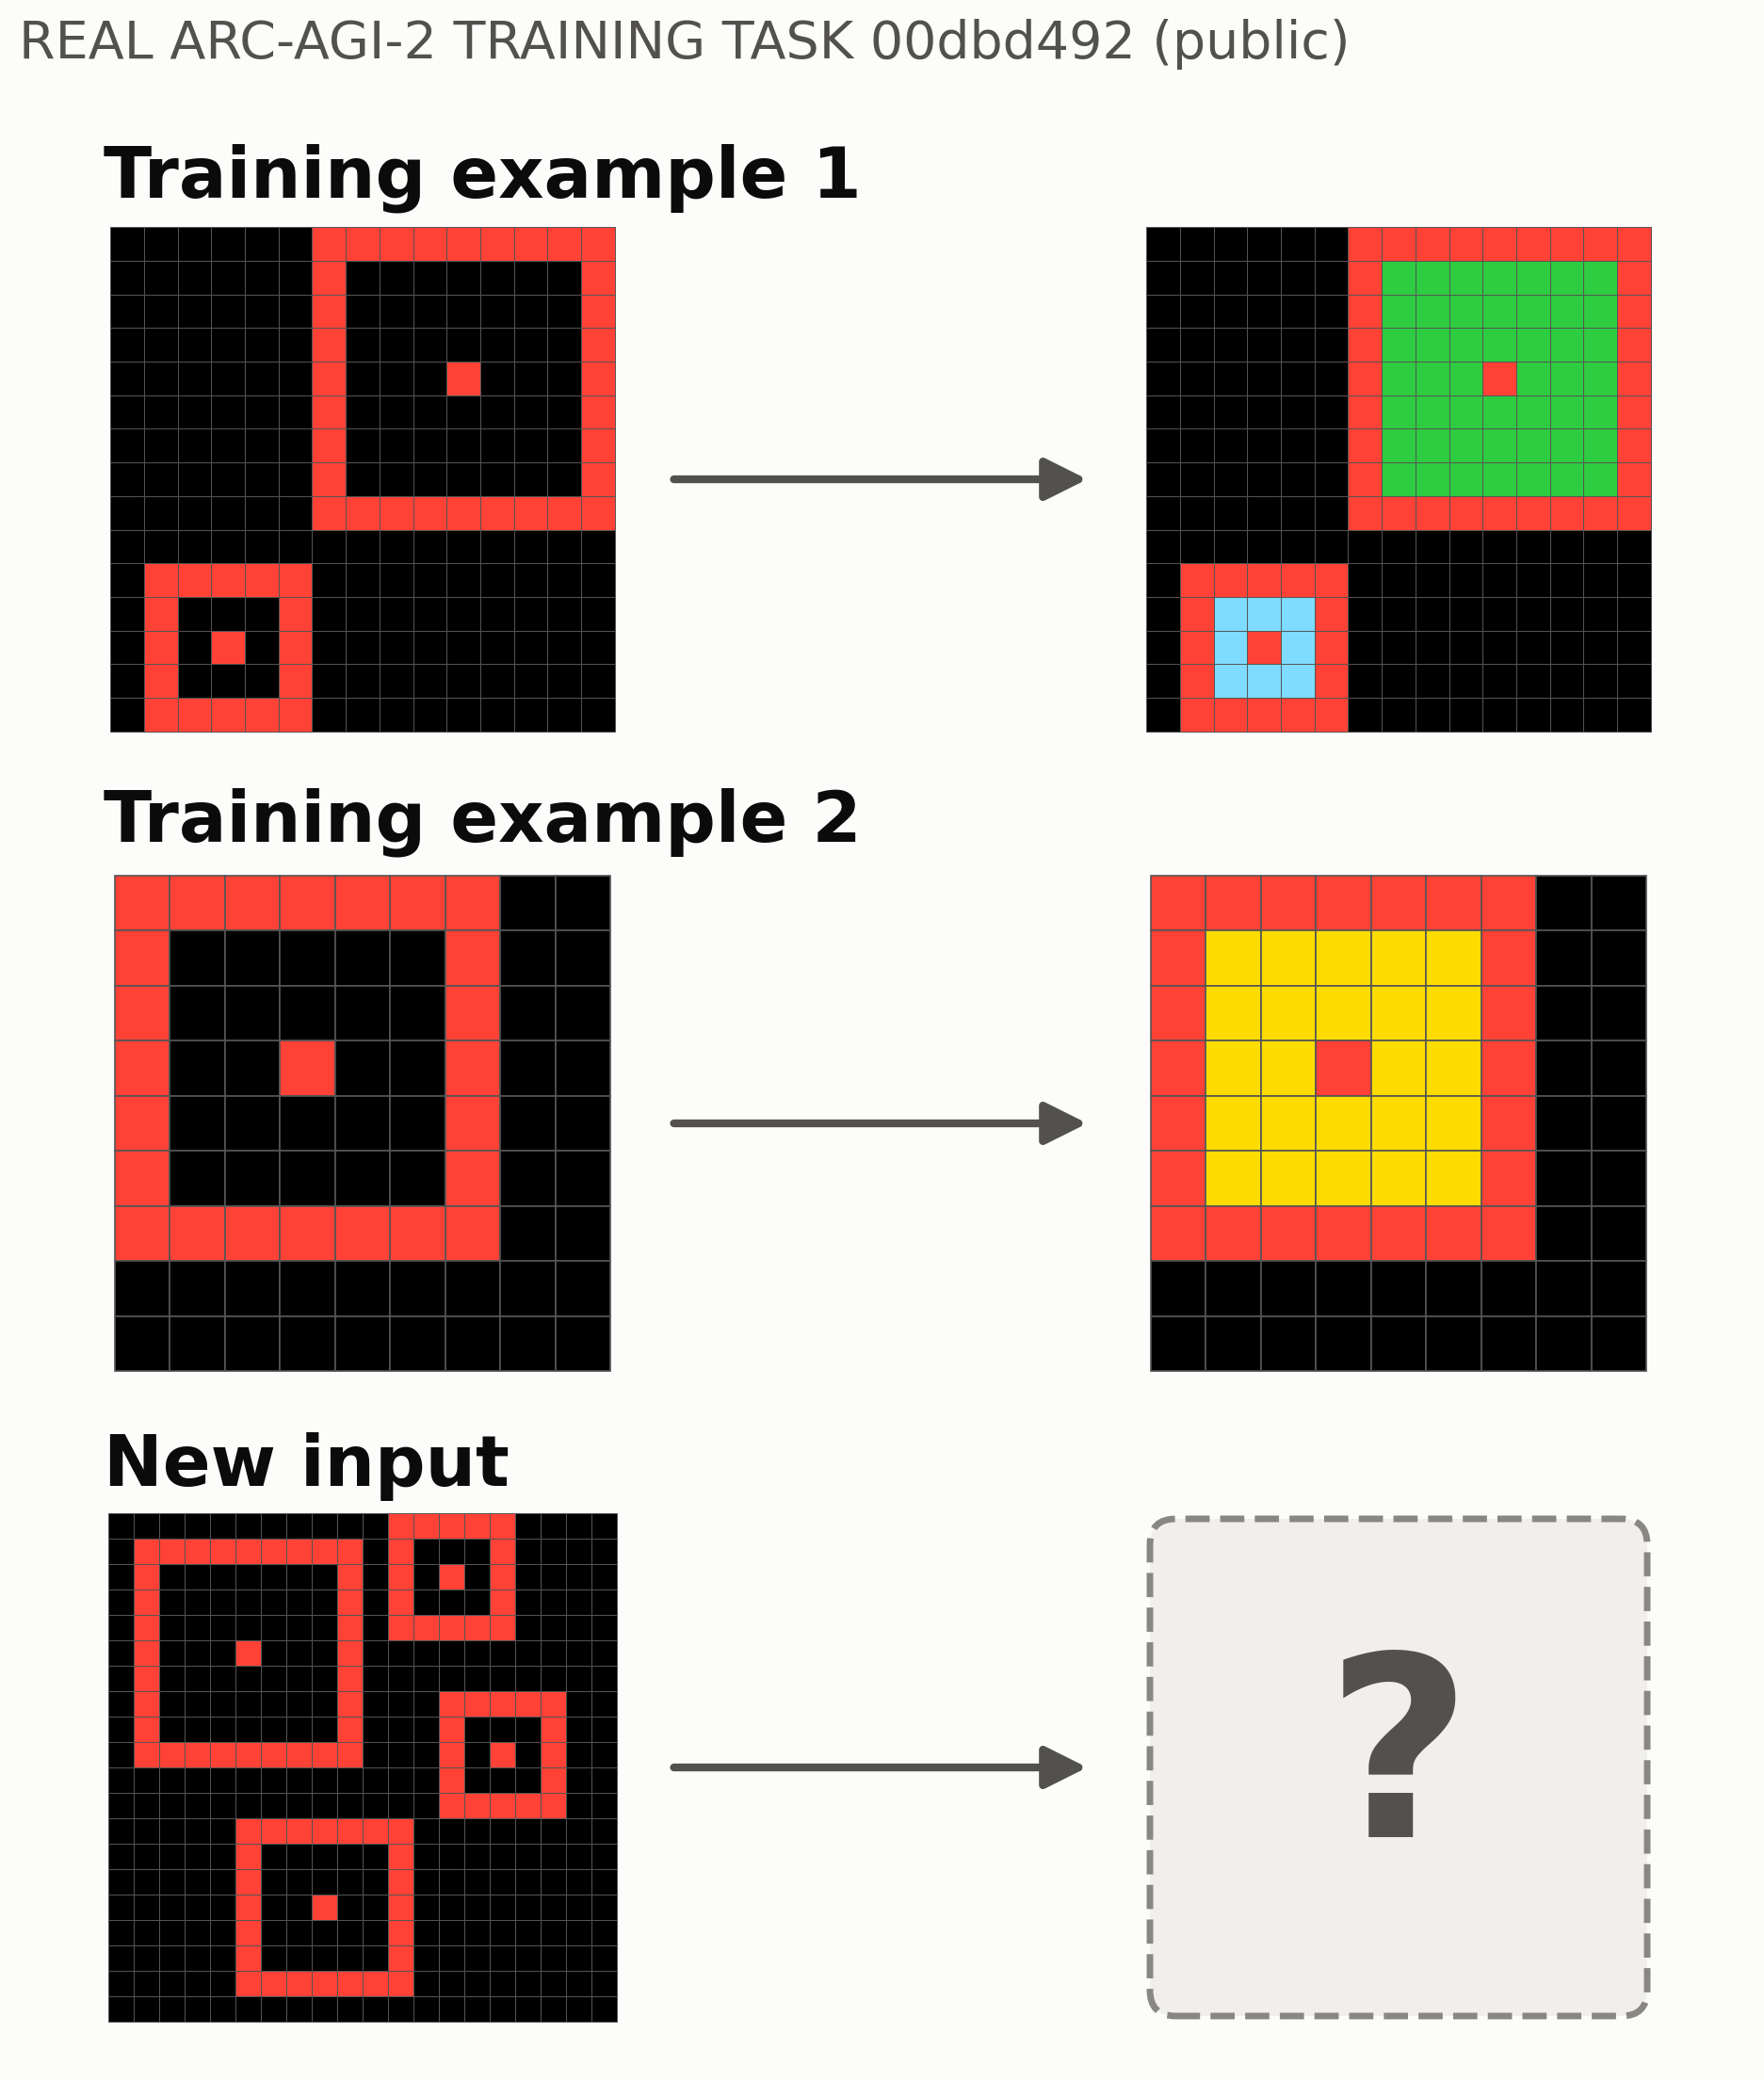
\includegraphics[width=0.66\linewidth]{figures/fig_arc_intro_00dbd492_large.png}
\caption{\label{fig:arc}A real public training task, 00dbd492, drawn cell for cell from the recorded bundle. Each frame is filled with a colour set by its size. The task was examined during development; here it only shows what an ARC task is.}
\end{figure}

\textbf{Memorization versus generalization.} "Paint the cells that changed in example 1" fits example 1 and fails elsewhere:
it memorizes. "Fill each frame with the colour its size calls for" generalizes. Both fit the demonstrations they were
built from, and that is the difficulty: fitting is not explaining.

\begin{figure}[H]
\centering
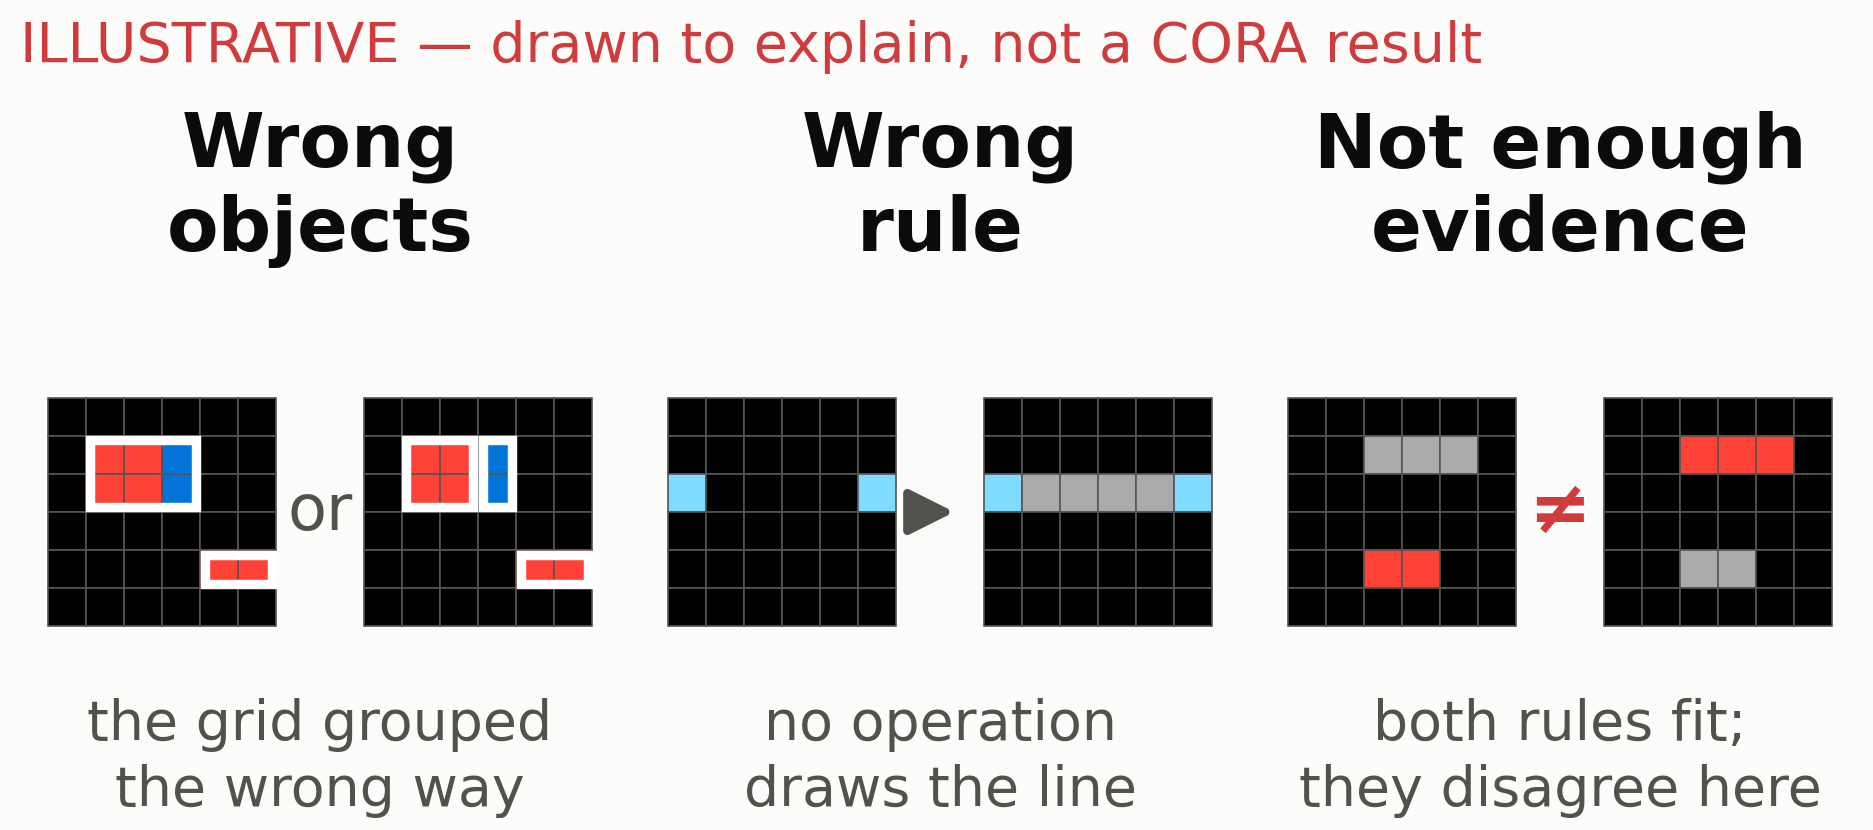
\includegraphics[width=\linewidth]{figures/fig_three_causes_row_ILLUSTRATIVE.png}
\caption{\label{fig:causes}ILLUSTRATIVE: three possible causes of a failed explanation, drawn to explain, not ARC tasks and not CORA results. Wrong objects: the same grid splits into two or three objects. Wrong rule: the available operations (move, recolour) cannot draw the line. Not enough evidence: "bars of two turn red" and "the top bar turns red" fit the same example and disagree on a new input.}
\end{figure}

\section{What CORA implements today}
\label{sec-cora}
CORA is an executable reasoner. Every hypothesis is a program that a fixed interpreter runs on the demonstrations.

\begin{itemize}
\item \textbf{Native CORA (frozen v23).} It segments a grid into objects in seven views, searches for an object program
(select objects, then keep, delete, recolour, move, copy, grow, \ldots{}), and accepts only programs that reproduce every
demonstration and are rebuilt when each demonstration is held out in turn.
\item \textbf{Rule construction (CORA-FHR, failure-conditioned hypothesis revision).} It reads native's own failure trace and
constructs a missing growth operation from a fixed typed grammar of 37,750 expressions. It installs the operation
reversibly and keeps it only if the unchanged engine uses it and every held-out fold rebuilds it.
\item \textbf{CORA-v2, the hypothesis reasoner.} It keeps every hypothesis (representation, geometry, colour policy) that
reproduces every demonstration. It abstains when they disagree, reruns the search with each demonstration held out,
and labels \textbf{why} it is unsure with observable diagnoses. Exploratory guesses are kept apart from certified answers.
\item \textbf{Present versus proposed.} Solid in figure \ref{fig:pipeline}: objects, executable rules, execution, the support check,
the tested revision and the separate evaluator. Dashed: choosing which revision to make, and any learned prior.
\end{itemize}

\section{Recorded evidence: a rule CORA built}
\label{sec-witness}
\begin{figure}[H]
\centering
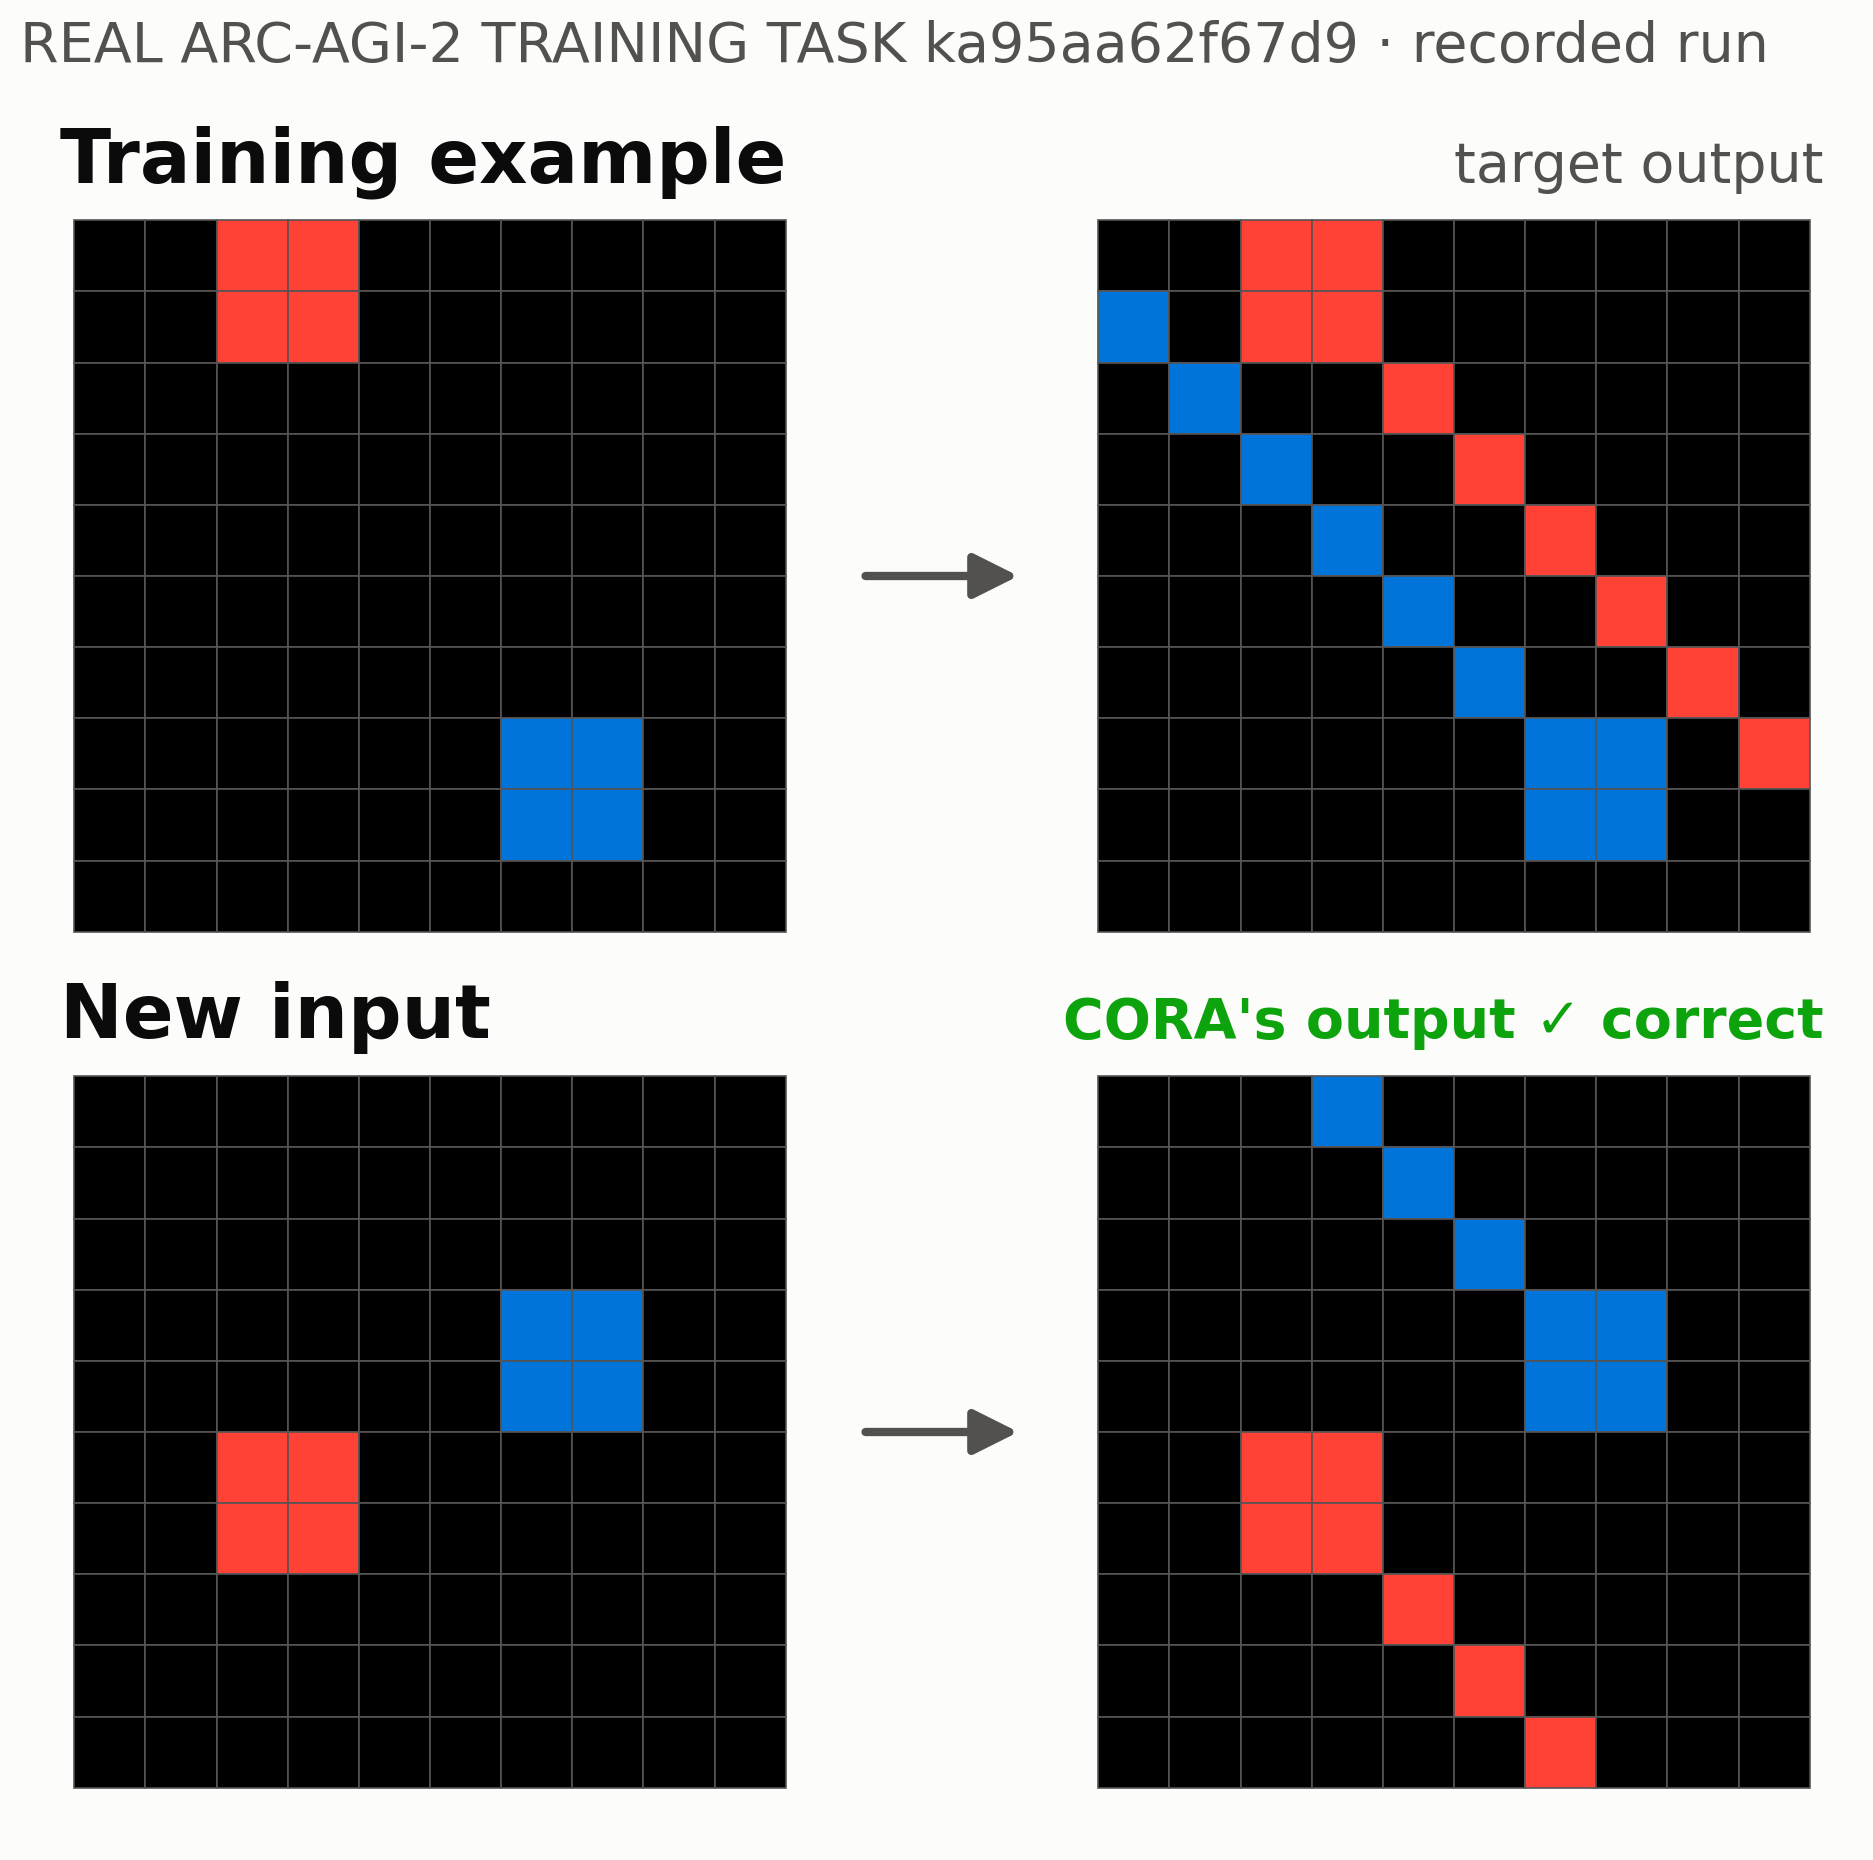
\includegraphics[width=0.74\linewidth]{figures/fig_real_rule_ka95aa62f67d9_large.png}
\caption{\label{fig:ka95}Real grids from the recorded bundle of task ka95aa62f67d9 (a training example with its target output; the new input with CORA's output, which equals the evaluator's answer).}
\end{figure}

\begin{itemize}
\item \textbf{The rule CORA constructed.} If an object's colours are \{1\}, a ray goes north-west from its centre to the border;
otherwise south-east. In ARC colours: \textbf{blue objects send a line up-left, red objects down-right}, each in the object's
own colour.
\item \textbf{The checks.} The rule was installed reversibly in the unchanged engine and rebuilt in 3 of 3 held-out folds. Its
output equals the evaluator's answer. Frozen native CORA and matched extra search do not solve this task.
\item \textbf{Why it is narrow.} The task was chosen in development by a failure autopsy, and it is an exposed public training task.
A constructor that ignored the failure record found the same rule. So the run shows that CORA can \textbf{construct and verify}
a missing rule. It does not show that diagnosing the failure \textbf{caused} the gain.
\item \textbf{The offline demo} (\texttt{sh docs/summit\_demo\_20261023/run\_demo.sh -{}-{}real}) replays the recorded run and re-executes the
constructed operation as standalone code. It is not a live rerun of the full engine.
\end{itemize}

\section{Negative evidence and the measured bottleneck}
\label{sec-negative}
\begin{figure}[H]
\centering
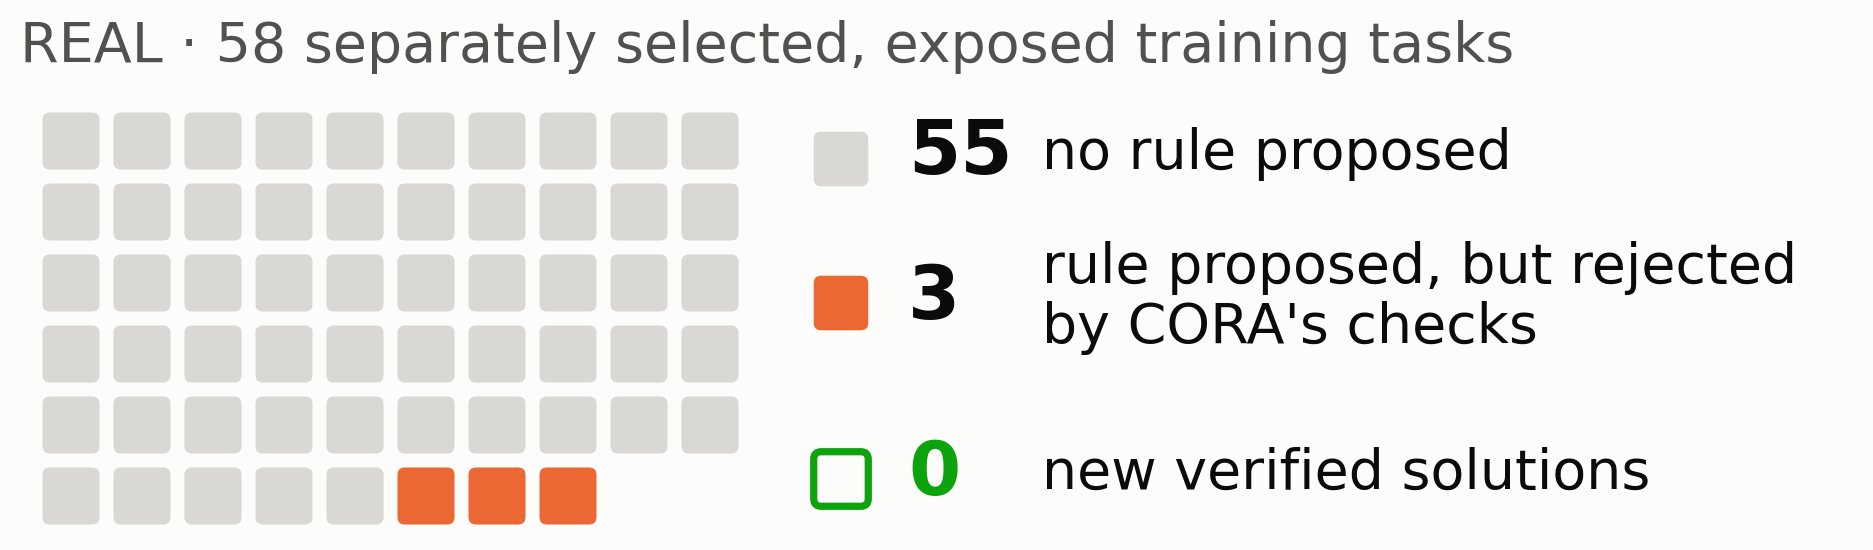
\includegraphics[width=0.95\linewidth]{figures/fig_construction_58_outcomes.png}
\caption{\label{fig:58}The 58-task generalization test of rule construction, one square per task, for the arm that used the failure record. No rule was proposed on 55 tasks; on 3, a rule was proposed but rejected (2 by the unchanged engine, 1 by the held-out rebuild); 0 verified.}
\end{figure}

\begin{itemize}
\item \textbf{The 58-task test.} 58 separately selected, still exposed training tasks, under a protocol frozen before the run. No
construction arm (with the failure record, failure-blind, shuffled, contrast) produced a verified new answer: 0 of 58,
with 0 wrong and 0 lost. The failure-blind arm: 52 no rule, 5 engine rejections, 1 held-out failure. Frozen native
solved 1, which is not a construction result.
\item \textbf{A restricted check on why.} An evaluator-only analysis, which reads the answers and is used only for diagnosis, asked
whether a \textbf{single, uniformly applied} growth expression could explain the changed cells in any of native's seven
views. For 50 of 58 tasks it could not. This supports an expressivity hypothesis inside that one class. It does not
show that the tasks need new semantics or are impossible for CORA.
\item \textbf{Fitting is not enough, measured.} On 60 exposed development tasks, CORA's object reasoner accepted 6 answers, all
correct. On 26 tasks every rule that fit the demonstrations failed the test (figure \ref{fig:dev60}).
\item \textbf{Thin evidence, flagged.} CORA-v2 certified no answer on 118 exposed development tasks; its exploratory guesses were 4
correct and 1 wrong. On 00dbd492 its 1,365 consistent hypotheses agree and the guess is correct, but the colour for
the largest frame is shown by one demonstration only. Hidden, that demonstration leaves the rebuilt rule without an
answer, so v2 keeps the guess uncertified (figure \ref{fig:v2}).
\item \textbf{Phase 2a (finished and evaluated, NO-GO).} On 40 freshly selected public training tasks, frozen native and matched
search each certified 6 answers (5 correct, 1 wrong). CORA-v2 certified none; its 2 exploratory answers were correct,
one of them new. The frozen GO rule needed 2 new correct answers, so the version was closed without retuning. On 33
of the 40 tasks no hypothesis in v2's language fit at all: the same bottleneck.
\end{itemize}

\begin{figure}[H]
\centering
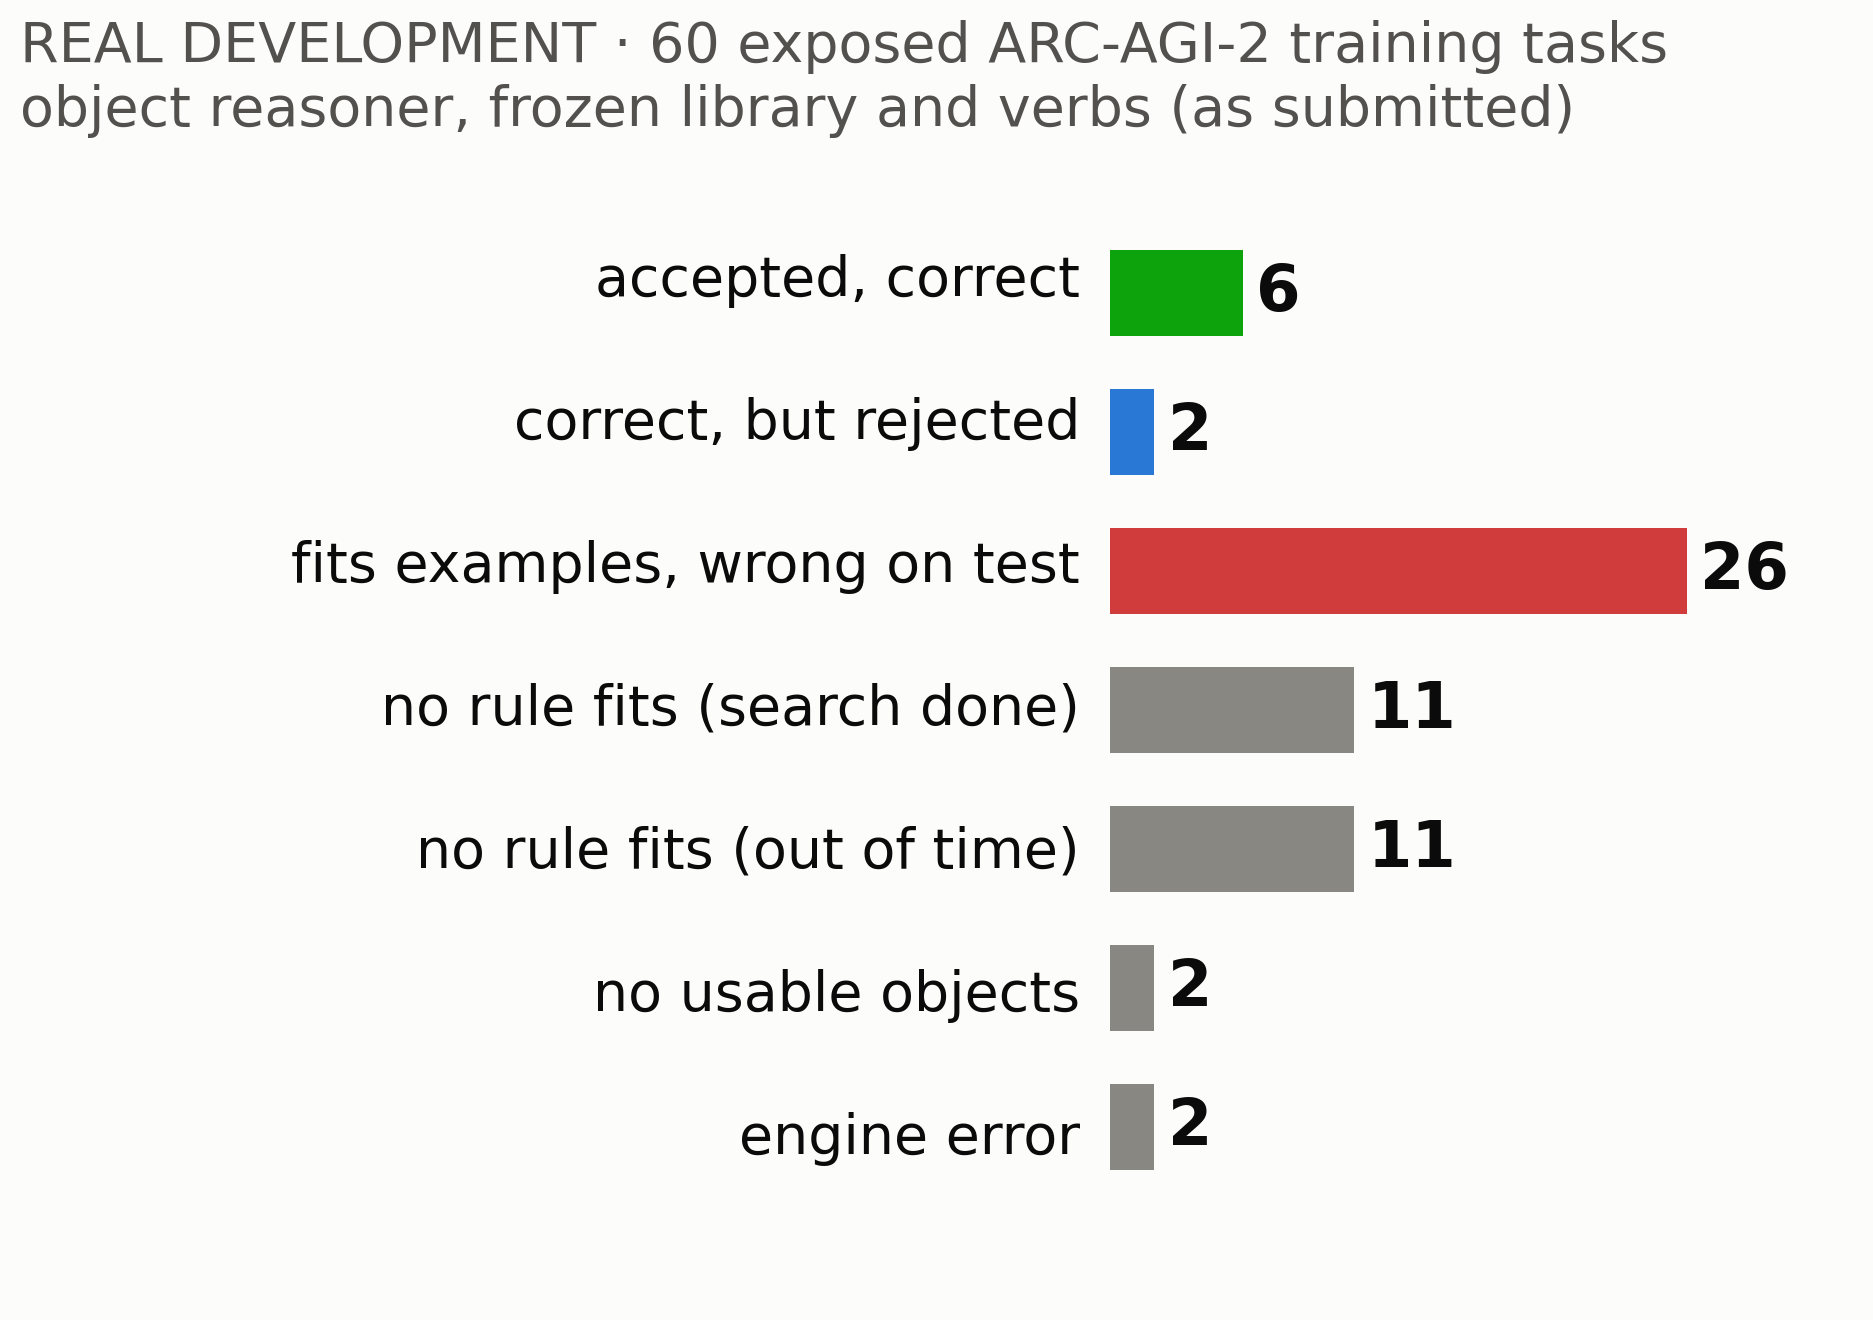
\includegraphics[width=0.85\linewidth]{figures/fig_dev60_audit_assets.png}
\caption{\label{fig:dev60}The 60-task audit of native CORA's object reasoner, as submitted, on exposed training tasks. This is one branch; the whole harness solved 12 of 60 over two attempts.}
\end{figure}

\begin{figure}[H]
\centering
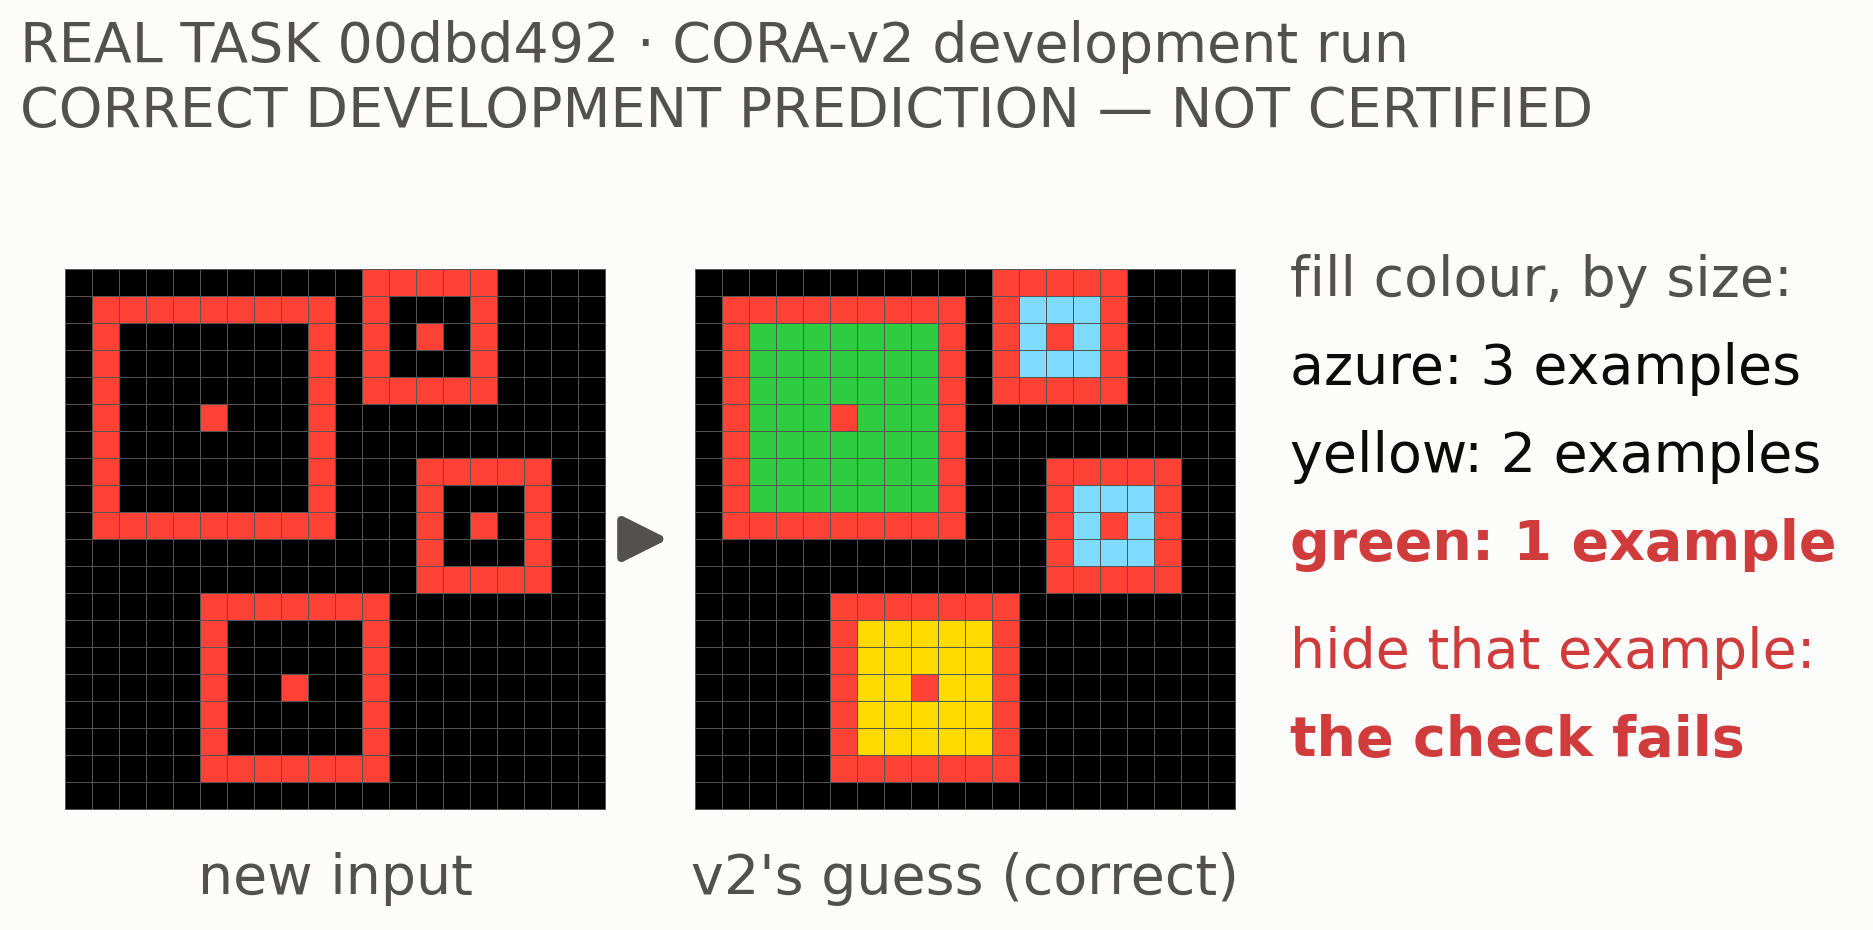
\includegraphics[width=0.9\linewidth]{figures/fig_v2_uncertified_00dbd492_large.png}
\caption{\label{fig:v2}CORA-v2 on 00dbd492 (development run): a correct but uncertified prediction. The fill colour for the largest frame rests on one demonstration.}
\end{figure}

\section{Why NVARC, and why neural learning}
\label{sec-nvarc}
\begin{itemize}
\item \textbf{What was reproduced.} NVARC is the NVARC team's published ARC Prize 2025 method. I deployed their public notebook with
six changes, all for deployment (compatibility, coverage, diagnostics, provenance, robustness). Unchanged: their
Qwen3-4B checkpoint, their per-task test-time training, decoding, scoring and selection.
\item \textbf{What Qwen learned in that method.} For each task, NVARC briefly trains a small adapter on the task's demonstrations
(eight rotations and reflections × sixteen colour permutations), then decodes and scores candidate grids. This is
learning within a task; the model emits grids, not programs.
\item \textbf{Attribution.} 27.64\% is the official public score of my deployment of their method (Kaggle 57160429). It is not a CORA
result and not a Neural-CORA result. Native CORA and CORA with rule construction scored 0.00\% (57144804, 57354496).
\item \textbf{Why combining answers failed.} On 240 exposed stand-in tasks, NVARC got 248 of 259 outputs and CORA 47; CORA solved
none that NVARC missed. Filling NVARC's empty second attempts with CORA's answers gained 0 and lost 1. On the hidden set
CORA scored 0.00, so its grids could add nothing there.
\item \textbf{An earlier neural negative.} A frozen, prompted Qwen2.5-1.5B that ranked CORA's seven segmentation views did not beat
a fixed order (35 of 35 against 19), and failure traces made it worse (1 of 35, the same as shuffled traces).
\item \textbf{Why a trained prior inside CORA is a different hypothesis.} It would be trained, not prompted. It would order a
search space of thousands to millions of typed programs, where no fixed order can be best for everything, instead of
choosing one of seven views. It uses no failure traces, and it must beat strong symbolic search under matched
compute.
\end{itemize}

\section{The proposed single Neural-CORA architecture}
\label{sec-neural}
One inference algorithm, owned by CORA; not a router, an ensemble or a second-attempt filler (figure \ref{fig:neural}).

\begin{figure}[H]
\centering
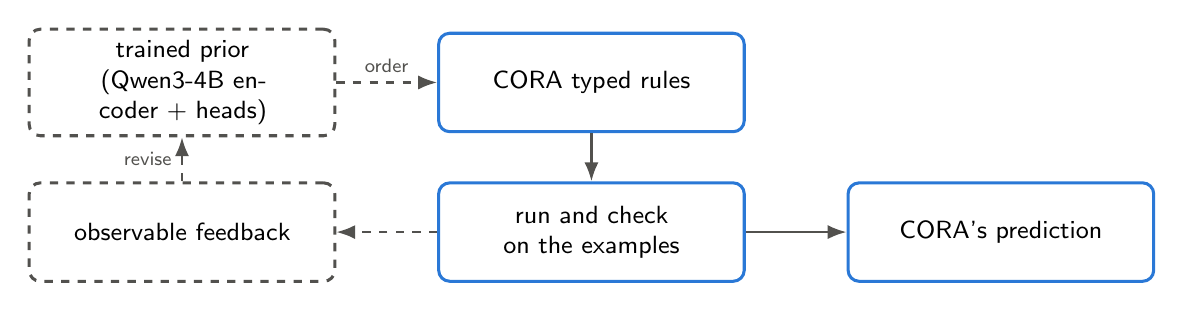
\begin{tikzpicture}
  \tikzset{n/.style={stage, text width=3.6cm}, pn/.style={pstage, text width=3.6cm}}
  \node[pn] (a) at (0,0) {trained prior\\(Qwen3-4B encoder + heads)};
  \node[n] (b) at (5.2,0) {CORA typed rules};
  \node[n] (c) at (5.2,-1.9) {run and check on the examples};
  \node[pn] (d) at (0,-1.9) {observable feedback};
  \node[n] (e) at (10.4,-1.9) {CORA's prediction};
  \draw[dflow] (a) -- node[above, font=\scriptsize, text=ink2] {order} (b); \draw[flow] (b) -- (c); \draw[dflow] (c) -- (d);
  \draw[dflow] (d) -- node[left, font=\scriptsize, text=ink2] {revise} (a); \draw[flow] (c) -- (e);
\end{tikzpicture}
\caption{\label{fig:neural}The proposed learning component inside CORA. Solid: CORA's existing typed rules, interpreter and prediction. Dashed: the trained prior and the feedback that would revise it; not yet validated.}
\end{figure}

\begin{itemize}
\item \textbf{CORA's typed state:} representation (a segmentation view), one or two first-match rules (selector and native action,
additive or not), a default, and the evidence: which demonstrations fit, fold outcomes, rival predictions, cost.
\item \textbf{The trainable prior:} the frozen NVARC Qwen3-4B checkpoint reads the demonstrations in its own grid format. A small
trainable head turns its hidden states into scores over program components. The scores only \textbf{order} CORA's search.
\item \textbf{Execution and selection:} the unchanged native interpreter runs each candidate; the same fixed rule picks two
attempts for every arm. No neural grid reaches an attempt.
\item \textbf{Fold-locality:} a prior adapted on all demonstrations cannot certify a fold; its proposals are labelled
neural-assisted unless the adaptation is repeated without the held-out demonstration.
\item \textbf{Status, 19 October:} the typed language compiles to native programs and runs through the native interpreter; CORA's
own synthetic task generator (execution-validated, no third-party data) and the arms are implemented, with unit tests.
A small engineering dry run is under way. \textbf{There is no result.} The pilot protocol is frozen before any scored run.
\end{itemize}

\section{How the idea could be falsified}
\label{sec-falsify}
Every arm uses the same inputs, the same interpreter and the same checker:

\begin{center}
\begin{tabularx}{\linewidth}{lYY}
arm & what it is & what it controls\\[0pt]
\hline
C0 & native CORA's own inducer & the original system\\[0pt]
C+ & simplest-first search, twice the learned budget & extra symbolic search\\[0pt]
C+H & C+ plus a hand-designed analysis of the changes & strong symbolic search\\[0pt]
L0, L0s & the same prior untrained, or trained on shuffled targets & does training matter?\\[0pt]
L1 & the trained prior & the hypothesis\\[0pt]
L1h & the same heads on hand-crafted features & does the neural encoder matter?\\[0pt]
N0, N+ & unchanged NVARC; NVARC with matched extra compute & the neural baseline (later stages)\\[0pt]
\end{tabularx}
\end{center}

Three outcomes must be kept apart: \textbf{candidate coverage} (a correct program is proposed at all), \textbf{exact accuracy} (the two
attempts are right), and \textbf{diagnostic benefit} (authentic feedback chooses revisions better than blind or shuffled
feedback). If the trained prior cannot beat C+ under matched resources on held-out task families, the result is NO-GO
and the bottleneck is diagnosed before any larger model is trained.

\section{People and the broader programme}
\label{sec-people}
\begin{itemize}
\item \textbf{Toni Kazic.} The general question at the top of the poster was discussed with Toni in a recorded conversation
(transcript: \texttt{voice\_note/arc\_conversatn.md}). The poster's wording is the author's; Toni's preferred wording is to be
confirmed.
\item \textbf{Chris.} The 2025 ARC work with Chris (the slides list Christian Fluharty, Computer Science, as co-presenter;
identity and naming to be confirmed) used LLM proposals with a program language, which this work builds on in spirit.
\item \textbf{Pierce Taylor.} A joint project with Pierce and Toni exists (\texttt{sb\_class\_project}). Its description, and any biological
test of a revision procedure, await Pierce's review. No conclusion from it is reported here.
\item \textbf{What could transfer} is the revision policy and the verification discipline, not ARC operations. Biology remains
future, untested work.
\end{itemize}

\section{Reproduction, terms and responsible claims}
\label{sec-repro}
\begin{itemize}
\item \textbf{Figures:} \texttt{python scripts/summit\_visual\_figures.py} (stops if any pinned input's hash differs); provenance in
\texttt{figures/PROVENANCE.json}.
\item \textbf{This explainer and the poster:} \texttt{sh scripts/build\_summit\_org.sh all} exports each \texttt{.org} to \LaTeX{} with Emacs and
compiles that export; \texttt{sh scripts/build\_summit\_org.sh selftest} proves the \texttt{.org} files are the real sources. Details:
\texttt{ORG\_TO\_PDF\_README.md}.
\item \textbf{Records:} the claim ledger; \texttt{records/CORA\_REASONING\_V2\_PHASE2A\_EXECUTION\_20261019.md};
\texttt{records/NEURAL\_CORA\_ARCHITECTURE\_AUDIT\_20261019.md}.
\end{itemize}

\textbf{Terms kept off the poster.} \emph{Leave-one-out} (LOO): rebuild a rule with one demonstration hidden and check that it
predicts it. \emph{Certified}: unique and rebuilt in every fold. \emph{Exploratory}: fits every demonstration but is not certified.
\emph{FHR}: failure-conditioned hypothesis revision. \emph{Grammar} or \emph{rule language}: what a system can express at all. \emph{K2} and
\emph{Step B}: a separate CORA experiment on inventing new operations, not used here. \emph{Oracle}: an evaluator-only analysis
that reads answers for diagnosis only. \emph{OOD}: tasks unlike those used in development. \emph{Causal claim}: a component caused
a gain, shown only by a controlled comparison. \emph{Exposed task}: already examined in development, so results on it are
in-sample. \emph{Version space}: every hypothesis consistent with the demonstrations.

\textbf{Credits and disclosure.} Authorship and credits are pending review by Toni, Chris and Pierce. AI coding assistance was
used for parts of the implementation and documentation; the research, decisions and claims are the author's.
\end{document}
